%\section{Mixed Team Tournament}
%\label{sec:mixedTeamTournament}
%This section contains all rules regarding the mixed teams tournament.
%
%For the 2019 tournament, pairs of teams will announce their partnership as part of the answer to the official call for application, as in last year's application. As part of the application, potential team pairs should announce the name of the second team, the mixed team name, and their proposed jersey color. Teams are strongly encouraged to change their mixed team partner from the previous year to spread the communication and behavior advancements.
%
%\subsection{Limitations}
%In 2019, the tournament will be limited to eight mixed teams. Both teams comprising a mixed team should run their own codebase, but are encouraged to develop a layer for interoperability which could later be used to form mixed teams with other teams.

%\subsection{Process of the Tournament}
%The tournament will be played 6 vs 6 on a regular SPL field. Besides the number of players, all other normal SPL rules apply.
%
%For the 2019 tournament, there will be 11 games in total: a round robin phase of 5 teams with 10 games and a championship game. Hence, each mixed team would play a total of 4 or 5 games in the mixed team tournament.
%
%If a penalty shootout is necessary after the group phase or in the final games, the following robot selection procedure will apply in order, where the home team consists of individual teams A and B, and the away team consists of the individual teams C and D:
%
%\begin{enumerate}
%  \item Striker A vs Goalie C
%  \item Striker C vs Goalie B
%  \item Striker B vs Goalie D
%  \item Striker D vs Goalie A
%  \item Striker A vs Goalie D
%  \item Striker C vs Goalie A
%  \item Striker B vs Goalie C
%  \item Striker D vs Goalie B
%\end{enumerate}
%
%If after these eight penalty kicks the result is still even, the teams will continue with the standard sudden-death shootout procedure (\cf Section~\ref{sec:sudden_death_shoot_out}) and may select the participating robot for each kick from both individual teams.

\newpage
\section{General Penalty Kick Challenge}
\label{sec:generalPenaltyKickChallenge}
This section contains the rules for the General Penalty Kick Challenge.

The rules are a slightly modified version of the usual penalty shootout rules.

\subsection{Process of the Tournament}
The challenge will be held as a single elimination tournament.
\begin{itemize}
  \item One Pre Top 16 round, consisting of all teams exclusive Top 8 of last
  year's competition.
  \item One Top 16 round, consisting of the top teams and winners of the Pre
  Top 16 round.
  \item The Top 8 round.
  \item The Top 4 round.
  \item The Final.
\end{itemize}

It is mandatory to provide two referees per team for the challenge.
The winner of the challenge will be awarded with a certificate.
The challenge will be held the day before the official competition starts.
A schedule will be announced for match-makers and referees. Teams must hand their robots to the referees within 2 minutes of the previous penalty shoot-out concluding. No late robots will be accepted. Referees scheduled for the next shoot-out must be at the field and ready to referee when the previous shoot-out ends.

Violations of any of these rules will be recorded and may affect future qualifications.

\begin{figure}[ht]
  \centerline{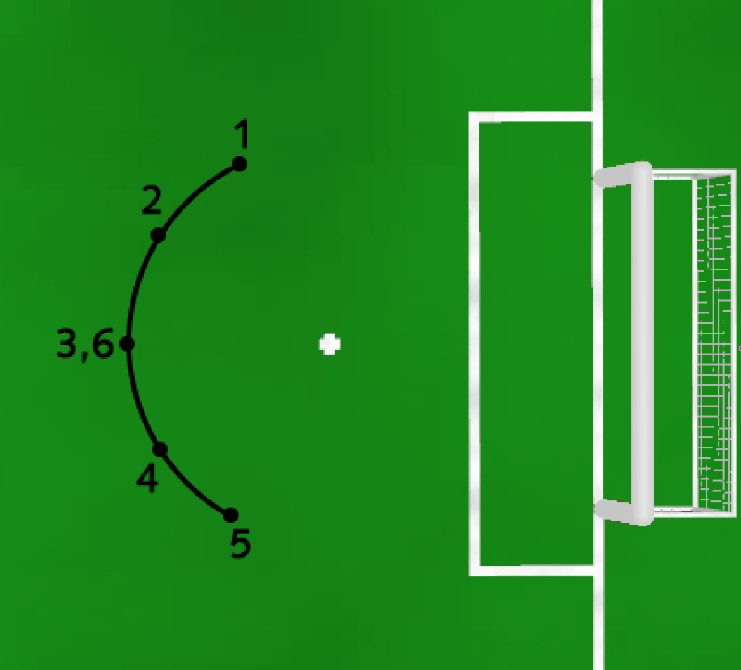
\includegraphics[width=0.5\columnwidth]{figs/general_penalty_setup}}
  \caption{Possible striker positions for the General Penalty Kick Challenge.}
  \label{fig:general_penalty_setup}
\end{figure}

\subsection{Rule Modifications}
The striker is positioned on a circle segment of radius 1m and an opening angle of $120^\circ$ around the penalty spot facing the ball. On this circle segment two spots to the left and two spots to the right with a distance of each $30^\circ$ are marked as starting position (see Figure~\ref{fig:general_penalty_setup}). For each round each team has to hand over one striker and one goalkeeper or just one robot if goalkeeper and striker are the same robot. Afterwards the head referee throws a die to determine the starting position as in Figure~\ref{fig:general_penalty_setup} for this round).
